\documentclass[twoside]{book}

% Packages required by doxygen
\usepackage{fixltx2e}
\usepackage{calc}
\usepackage{doxygen}
\usepackage[export]{adjustbox} % also loads graphicx
\usepackage{graphicx}
\usepackage[utf8]{inputenc}
\usepackage{makeidx}
\usepackage{multicol}
\usepackage{multirow}
\PassOptionsToPackage{warn}{textcomp}
\usepackage{textcomp}
\usepackage[nointegrals]{wasysym}
\usepackage[table]{xcolor}

% NLS support packages
\usepackage[french]{babel}

% Font selection
\usepackage[T1]{fontenc}
\usepackage[scaled=.90]{helvet}
\usepackage{courier}
\usepackage{amssymb}
\usepackage{sectsty}
\renewcommand{\familydefault}{\sfdefault}
\allsectionsfont{%
  \fontseries{bc}\selectfont%
  \color{darkgray}%
}
\renewcommand{\DoxyLabelFont}{%
  \fontseries{bc}\selectfont%
  \color{darkgray}%
}
\newcommand{\+}{\discretionary{\mbox{\scriptsize$\hookleftarrow$}}{}{}}

% Page & text layout
\usepackage{geometry}
\geometry{%
  a4paper,%
  top=2.5cm,%
  bottom=2.5cm,%
  left=2.5cm,%
  right=2.5cm%
}
\tolerance=750
\hfuzz=15pt
\hbadness=750
\setlength{\emergencystretch}{15pt}
\setlength{\parindent}{0cm}
\setlength{\parskip}{3ex plus 2ex minus 2ex}
\makeatletter
\renewcommand{\paragraph}{%
  \@startsection{paragraph}{4}{0ex}{-1.0ex}{1.0ex}{%
    \normalfont\normalsize\bfseries\SS@parafont%
  }%
}
\renewcommand{\subparagraph}{%
  \@startsection{subparagraph}{5}{0ex}{-1.0ex}{1.0ex}{%
    \normalfont\normalsize\bfseries\SS@subparafont%
  }%
}
\makeatother

% Headers & footers
\usepackage{fancyhdr}
\pagestyle{fancyplain}
\fancyhead[LE]{\fancyplain{}{\bfseries\thepage}}
\fancyhead[CE]{\fancyplain{}{}}
\fancyhead[RE]{\fancyplain{}{\bfseries\leftmark}}
\fancyhead[LO]{\fancyplain{}{\bfseries\rightmark}}
\fancyhead[CO]{\fancyplain{}{}}
\fancyhead[RO]{\fancyplain{}{\bfseries\thepage}}
\fancyfoot[LE]{\fancyplain{}{}}
\fancyfoot[CE]{\fancyplain{}{}}
\fancyfoot[RE]{\fancyplain{}{\bfseries\scriptsize Généré par Doxygen }}
\fancyfoot[LO]{\fancyplain{}{\bfseries\scriptsize Généré par Doxygen }}
\fancyfoot[CO]{\fancyplain{}{}}
\fancyfoot[RO]{\fancyplain{}{}}
\renewcommand{\footrulewidth}{0.4pt}
\renewcommand{\chaptermark}[1]{%
  \markboth{#1}{}%
}
\renewcommand{\sectionmark}[1]{%
  \markright{\thesection\ #1}%
}

% Indices & bibliography
\usepackage{natbib}
\usepackage[titles]{tocloft}
\setcounter{tocdepth}{3}
\setcounter{secnumdepth}{5}
\makeindex

% Hyperlinks (required, but should be loaded last)
\usepackage{ifpdf}
\ifpdf
  \usepackage[pdftex,pagebackref=true]{hyperref}
\else
  \usepackage[ps2pdf,pagebackref=true]{hyperref}
\fi
\hypersetup{%
  colorlinks=true,%
  linkcolor=blue,%
  citecolor=blue,%
  unicode%
}

% Custom commands
\newcommand{\clearemptydoublepage}{%
  \newpage{\pagestyle{empty}\cleardoublepage}%
}

\usepackage{caption}
\captionsetup{labelsep=space,justification=centering,font={bf},singlelinecheck=off,skip=4pt,position=top}

%===== C O N T E N T S =====

\begin{document}

% Titlepage & ToC
\hypersetup{pageanchor=false,
             bookmarksnumbered=true,
             pdfencoding=unicode
            }
\pagenumbering{roman}
\begin{titlepage}
\vspace*{7cm}
\begin{center}%
{\Large projet mot mélés }\\
\vspace*{1cm}
{\large Généré par Doxygen 1.8.11}\\
\end{center}
\end{titlepage}
\clearemptydoublepage
\tableofcontents
\clearemptydoublepage
\pagenumbering{arabic}
\hypersetup{pageanchor=true}

%--- Begin generated contents ---
\chapter{Index des structures de données}
\section{Structures de données}
Liste des structures de données avec une brève description \+:\begin{DoxyCompactList}
\item\contentsline{section}{\hyperlink{structmat__s}{mat\+\_\+s} }{\pageref{structmat__s}}{}
\item\contentsline{section}{\hyperlink{structmot__mat__s}{mot\+\_\+mat\+\_\+s} }{\pageref{structmot__mat__s}}{}
\end{DoxyCompactList}

\chapter{Index des fichiers}
\section{Liste des fichiers}
Liste de tous les fichiers documentés avec une brève description \+:\begin{DoxyCompactList}
\item\contentsline{section}{src/{\bfseries direction.\+h} }{\pageref{direction_8h}}{}
\item\contentsline{section}{src/\hyperlink{generateur_8c}{generateur.\+c} \\*Generateur.\+c est un liste de fonction qui sont utilisé pour générer le mot mélés sur lesquels jouer }{\pageref{generateur_8c}}{}
\item\contentsline{section}{src/{\bfseries generateur.\+h} }{\pageref{generateur_8h}}{}
\item\contentsline{section}{src/\hyperlink{matrice_8c}{matrice.\+c} \\*Matrice.\+c comporte toute les fonction utiles a la gestion de la matrice }{\pageref{matrice_8c}}{}
\item\contentsline{section}{src/{\bfseries matrice.\+h} }{\pageref{matrice_8h}}{}
\item\contentsline{section}{src/\hyperlink{mot_8c}{mot.\+c} \\*Mot.\+c est un programme qui a les différentes fonction liés a la liste de mot de départ }{\pageref{mot_8c}}{}
\item\contentsline{section}{src/{\bfseries mot.\+h} }{\pageref{mot_8h}}{}
\item\contentsline{section}{src/\hyperlink{mot__mat_8c}{mot\+\_\+mat.\+c} \\*Mot\+\_\+mat.\+c permet de gerer les \hyperlink{mot__mat_8c}{mot\+\_\+mat.\+c} }{\pageref{mot__mat_8c}}{}
\item\contentsline{section}{src/{\bfseries mot\+\_\+mat.\+h} }{\pageref{mot__mat_8h}}{}
\item\contentsline{section}{src/\hyperlink{outil_8c}{outil.\+c} \\*Outil.\+c est une liste de fonction global (qu\textquotesingle{}on pourrais utilsier tel quel dans un autre programme }{\pageref{outil_8c}}{}
\item\contentsline{section}{src/{\bfseries outil.\+h} }{\pageref{outil_8h}}{}
\item\contentsline{section}{src/{\bfseries premier\+\_\+saisie.\+h} }{\pageref{premier__saisie_8h}}{}
\end{DoxyCompactList}

\chapter{Documentation des structures de données}
\hypertarget{structmat__s}{}\section{Référence de la structure mat\+\_\+s}
\label{structmat__s}\index{mat\+\_\+s@{mat\+\_\+s}}
\subsection*{Champs de données}
\begin{DoxyCompactItemize}
\item 
int {\bfseries nbc}\hypertarget{structmat__s_ae42929290738ae9582f3d72273b848de}{}\label{structmat__s_ae42929290738ae9582f3d72273b848de}

\item 
int {\bfseries nbl}\hypertarget{structmat__s_ad7880699540a3f2e94ed3ee7d5d3b320}{}\label{structmat__s_ad7880699540a3f2e94ed3ee7d5d3b320}

\item 
char $\ast$$\ast$ {\bfseries val}\hypertarget{structmat__s_a7a5b5d01a515e56fa0fb940202153cd1}{}\label{structmat__s_a7a5b5d01a515e56fa0fb940202153cd1}

\end{DoxyCompactItemize}


La documentation de cette structure a été générée à partir du fichier suivant \+:\begin{DoxyCompactItemize}
\item 
src/matrice.\+h\end{DoxyCompactItemize}

\hypertarget{structmot__mat__s}{}\section{Référence de la structure mot\+\_\+mat\+\_\+s}
\label{structmot__mat__s}\index{mot\+\_\+mat\+\_\+s@{mot\+\_\+mat\+\_\+s}}
\subsection*{Champs de données}
\begin{DoxyCompactItemize}
\item 
int {\bfseries colonne}\hypertarget{structmot__mat__s_a8d5fb219fa27d58faca17483f538a692}{}\label{structmot__mat__s_a8d5fb219fa27d58faca17483f538a692}

\item 
int {\bfseries ligne}\hypertarget{structmot__mat__s_ab6356d5fb49bcb2478ffab363e947e68}{}\label{structmot__mat__s_ab6356d5fb49bcb2478ffab363e947e68}

\item 
char $\ast$ {\bfseries mot}\hypertarget{structmot__mat__s_ae9144799389a5d8ba95e70dff6650adf}{}\label{structmot__mat__s_ae9144799389a5d8ba95e70dff6650adf}

\item 
t\+\_\+direction {\bfseries dir}\hypertarget{structmot__mat__s_a664c4d4a804890f1cbdff8a3923e1569}{}\label{structmot__mat__s_a664c4d4a804890f1cbdff8a3923e1569}

\end{DoxyCompactItemize}


La documentation de cette structure a été générée à partir du fichier suivant \+:\begin{DoxyCompactItemize}
\item 
src/mot\+\_\+mat.\+h\end{DoxyCompactItemize}

\chapter{Documentation des fichiers}
\hypertarget{generateur_8c}{}\section{Référence du fichier src/generateur.c}
\label{generateur_8c}\index{src/generateur.\+c@{src/generateur.\+c}}


\hyperlink{generateur_8c}{generateur.\+c} est un liste de fonction qui sont utilisé pour générer le mot mélés sur lesquels jouer  


{\ttfamily \#include \char`\"{}generateur.\+h\char`\"{}}\\*
Graphe des dépendances par inclusion de generateur.\+c\+:
\nopagebreak
\begin{figure}[H]
\begin{center}
\leavevmode
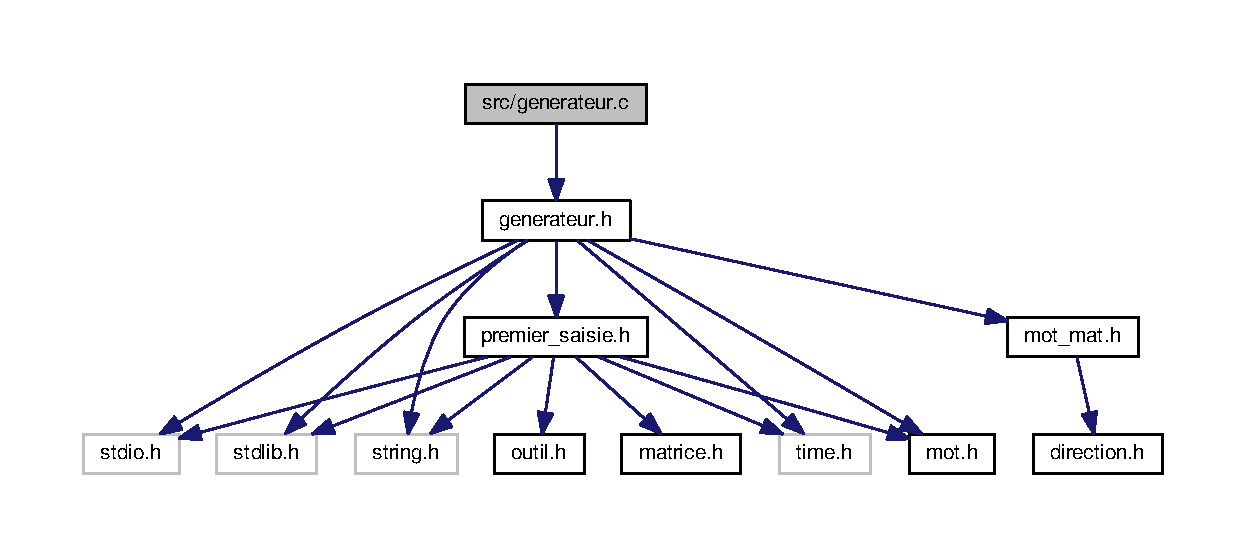
\includegraphics[width=350pt]{generateur_8c__incl}
\end{center}
\end{figure}
\subsection*{Fonctions}
\begin{DoxyCompactItemize}
\item 
int \hyperlink{generateur_8c_a968d1f30091e0590282aa664ffb64ab2}{coord\+\_\+valides} (int x, int y, \hyperlink{structmat__s}{mat\+\_\+t} ma\+\_\+mat)
\begin{DoxyCompactList}\small\item\em fonction qui vérifie que les coordonnées données sont possible dans la matrice donnée \end{DoxyCompactList}\item 
t\+\_\+direction \hyperlink{generateur_8c_adf533dc1f1f23ffd3878526a0ea66b85}{inserer} (char $\ast$mot, int i, int j, t\+\_\+direction direction, \hyperlink{structmat__s}{mat\+\_\+t} ma\+\_\+mat)
\begin{DoxyCompactList}\small\item\em insere dans la matrice donnéaux coordonnées avec la direction le mot \end{DoxyCompactList}\item 
\hyperlink{structmot__mat__s}{mot\+\_\+mat\+\_\+t} \hyperlink{generateur_8c_aee299ca0e78ef648178fe80ed386457b}{ajoutnonaleatoire} (\hyperlink{structmat__s}{mat\+\_\+t} ma\+\_\+mat)
\begin{DoxyCompactList}\small\item\em fonction qui insere bonjour en 7,6 direction est \end{DoxyCompactList}\item 
int \hyperlink{generateur_8c_ab013f83f7e6a5283d51b51e38e0cf407}{parcours\+\_\+libre} (int coordX, int coordY, t\+\_\+direction direction, \hyperlink{structmat__s}{mat\+\_\+t} ma\+\_\+mat, int version)
\begin{DoxyCompactList}\small\item\em fonction qui regarde la taille dans une direction donnée sans lettre \end{DoxyCompactList}\item 
\hyperlink{structmot__mat__s}{mot\+\_\+mat\+\_\+t} \hyperlink{generateur_8c_a879f01824fc254fe52a02bb2a8d08f08}{insert\+\_\+premier\+\_\+mot} (char $\ast$mot, int i1, int j1, t\+\_\+direction direction, \hyperlink{structmat__s}{mat\+\_\+t} ma\+\_\+mat)
\begin{DoxyCompactList}\small\item\em insere un mot sans verification \end{DoxyCompactList}\item 
\hyperlink{structmot__mat__s}{mot\+\_\+mat\+\_\+t} \hyperlink{generateur_8c_a3fb49352563af510db6f0498ef690ff7}{premier\+\_\+mot} (char $\ast$mot, \hyperlink{structmat__s}{mat\+\_\+t} ma\+\_\+mat)
\begin{DoxyCompactList}\small\item\em insere un mot avec des coordonnées et une direction alatoire \end{DoxyCompactList}\item 
\hyperlink{structmot__mat__s}{mot\+\_\+mat\+\_\+t} \hyperlink{generateur_8c_afa1a4981599a2b3aa429e0cf59b6324a}{Placerlibre} (\hyperlink{structmat__s}{mat\+\_\+t} ma\+\_\+mat)
\begin{DoxyCompactList}\small\item\em insere un mot,de la liste des mots,le plus grand possible à l\textquotesingle{}endroit le plus grand possible \end{DoxyCompactList}\item 
\hyperlink{structmot__mat__s}{mot\+\_\+mat\+\_\+t} {\bfseries Placer\+Mot} (\hyperlink{structmot__mat__s}{mot\+\_\+mat\+\_\+t} motmis, \hyperlink{structmat__s}{mat\+\_\+t} ma\+\_\+mat)\hypertarget{generateur_8c_aff3285f1fae64c682e5365ac6b4f8296}{}\label{generateur_8c_aff3285f1fae64c682e5365ac6b4f8296}

\item 
void \hyperlink{generateur_8c_a2f70c890274c026e3429547bce6e42aa}{remplir\+\_\+final} (\hyperlink{structmat__s}{mat\+\_\+t} ma\+\_\+mat)
\begin{DoxyCompactList}\small\item\em insere dans tout les endroits où il n\textquotesingle{}y a pas de lettre une lettre aléatoire \end{DoxyCompactList}\end{DoxyCompactItemize}


\subsection{Description détaillée}
\hyperlink{generateur_8c}{generateur.\+c} est un liste de fonction qui sont utilisé pour générer le mot mélés sur lesquels jouer 

... Documentation ...

\begin{DoxyAuthor}{Auteur}
T\+H\+O\+M\+AS Paul B\+E\+N\+J\+A\+M\+IN Matthey 
\end{DoxyAuthor}
\begin{DoxyVersion}{Version}
1.\+0 
\end{DoxyVersion}
\begin{DoxyDate}{Date}
3 avril 2018 
\end{DoxyDate}


\subsection{Documentation des fonctions}
\index{generateur.\+c@{generateur.\+c}!ajoutnonaleatoire@{ajoutnonaleatoire}}
\index{ajoutnonaleatoire@{ajoutnonaleatoire}!generateur.\+c@{generateur.\+c}}
\subsubsection[{\texorpdfstring{ajoutnonaleatoire(mat\+\_\+t ma\+\_\+mat)}{ajoutnonaleatoire(mat_t ma_mat)}}]{\setlength{\rightskip}{0pt plus 5cm}{\bf mot\+\_\+mat\+\_\+t} ajoutnonaleatoire (
\begin{DoxyParamCaption}
\item[{{\bf mat\+\_\+t}}]{ma\+\_\+mat}
\end{DoxyParamCaption}
)}\hypertarget{generateur_8c_aee299ca0e78ef648178fe80ed386457b}{}\label{generateur_8c_aee299ca0e78ef648178fe80ed386457b}


fonction qui insere bonjour en 7,6 direction est 


\begin{DoxyParams}{Paramètres}
{\em ma\+\_\+mat} & represente une matrice \\
\hline
\end{DoxyParams}
\begin{DoxyReturn}{Renvoie}
une variable de type mot\+\_\+mat\+\_\+t 
\end{DoxyReturn}
\index{generateur.\+c@{generateur.\+c}!coord\+\_\+valides@{coord\+\_\+valides}}
\index{coord\+\_\+valides@{coord\+\_\+valides}!generateur.\+c@{generateur.\+c}}
\subsubsection[{\texorpdfstring{coord\+\_\+valides(int x, int y, mat\+\_\+t ma\+\_\+mat)}{coord_valides(int x, int y, mat_t ma_mat)}}]{\setlength{\rightskip}{0pt plus 5cm}int coord\+\_\+valides (
\begin{DoxyParamCaption}
\item[{int}]{x, }
\item[{int}]{y, }
\item[{{\bf mat\+\_\+t}}]{ma\+\_\+mat}
\end{DoxyParamCaption}
)}\hypertarget{generateur_8c_a968d1f30091e0590282aa664ffb64ab2}{}\label{generateur_8c_a968d1f30091e0590282aa664ffb64ab2}


fonction qui vérifie que les coordonnées données sont possible dans la matrice donnée 


\begin{DoxyParams}{Paramètres}
{\em x} & la Coordonné X qui équivaut a la colonne ciblé \\
\hline
{\em y} & la Coordonné Y qui équivaut a la ligne ciblé \\
\hline
{\em ma\+\_\+mat} & represente une matrice \\
\hline
\end{DoxyParams}
\begin{DoxyReturn}{Renvoie}
vrai si les coordonnées sont valides faux sinon 
\end{DoxyReturn}
\index{generateur.\+c@{generateur.\+c}!inserer@{inserer}}
\index{inserer@{inserer}!generateur.\+c@{generateur.\+c}}
\subsubsection[{\texorpdfstring{inserer(char $\ast$mot, int i, int j, t\+\_\+direction direction, mat\+\_\+t ma\+\_\+mat)}{inserer(char *mot, int i, int j, t_direction direction, mat_t ma_mat)}}]{\setlength{\rightskip}{0pt plus 5cm}t\+\_\+direction inserer (
\begin{DoxyParamCaption}
\item[{char $\ast$}]{mot, }
\item[{int}]{i, }
\item[{int}]{j, }
\item[{t\+\_\+direction}]{direction, }
\item[{{\bf mat\+\_\+t}}]{ma\+\_\+mat}
\end{DoxyParamCaption}
)}\hypertarget{generateur_8c_adf533dc1f1f23ffd3878526a0ea66b85}{}\label{generateur_8c_adf533dc1f1f23ffd3878526a0ea66b85}


insere dans la matrice donnéaux coordonnées avec la direction le mot 


\begin{DoxyParams}{Paramètres}
{\em mot} & est un mot que l\textquotesingle{}on veut inserer \\
\hline
{\em i} & la Coordonné I qui équivaut a la colonne ciblé \\
\hline
{\em j} & la Coordonné J qui équivaut a la ligne ciblé \\
\hline
{\em direction} & est une direction \\
\hline
{\em ma\+\_\+mat} & represente une matrice \\
\hline
\end{DoxyParams}
\begin{DoxyReturn}{Renvoie}
la direction du mot qu\textquotesingle{}on a inserer 
\end{DoxyReturn}
\index{generateur.\+c@{generateur.\+c}!insert\+\_\+premier\+\_\+mot@{insert\+\_\+premier\+\_\+mot}}
\index{insert\+\_\+premier\+\_\+mot@{insert\+\_\+premier\+\_\+mot}!generateur.\+c@{generateur.\+c}}
\subsubsection[{\texorpdfstring{insert\+\_\+premier\+\_\+mot(char $\ast$mot, int i1, int j1, t\+\_\+direction direction, mat\+\_\+t ma\+\_\+mat)}{insert_premier_mot(char *mot, int i1, int j1, t_direction direction, mat_t ma_mat)}}]{\setlength{\rightskip}{0pt plus 5cm}{\bf mot\+\_\+mat\+\_\+t} insert\+\_\+premier\+\_\+mot (
\begin{DoxyParamCaption}
\item[{char $\ast$}]{mot, }
\item[{int}]{i1, }
\item[{int}]{j1, }
\item[{t\+\_\+direction}]{direction, }
\item[{{\bf mat\+\_\+t}}]{ma\+\_\+mat}
\end{DoxyParamCaption}
)}\hypertarget{generateur_8c_a879f01824fc254fe52a02bb2a8d08f08}{}\label{generateur_8c_a879f01824fc254fe52a02bb2a8d08f08}


insere un mot sans verification 


\begin{DoxyParams}{Paramètres}
{\em mot} & est me mot \\
\hline
{\em i1} & represente la la colonne ou l\textquotesingle{}on va commencer la recherche \\
\hline
{\em j1} & represente la la ligne ou l\textquotesingle{}on va commencer la recherche \\
\hline
{\em direction} & represente la direction ou l\textquotesingle{}on va inserer \\
\hline
{\em ma\+\_\+mat} & represente une matrice \\
\hline
\end{DoxyParams}
\begin{DoxyReturn}{Renvoie}
une variable de type mot\+\_\+mat\+\_\+t 
\end{DoxyReturn}
\index{generateur.\+c@{generateur.\+c}!parcours\+\_\+libre@{parcours\+\_\+libre}}
\index{parcours\+\_\+libre@{parcours\+\_\+libre}!generateur.\+c@{generateur.\+c}}
\subsubsection[{\texorpdfstring{parcours\+\_\+libre(int coord\+X, int coord\+Y, t\+\_\+direction direction, mat\+\_\+t ma\+\_\+mat, int version)}{parcours_libre(int coordX, int coordY, t_direction direction, mat_t ma_mat, int version)}}]{\setlength{\rightskip}{0pt plus 5cm}int parcours\+\_\+libre (
\begin{DoxyParamCaption}
\item[{int}]{coordX, }
\item[{int}]{coordY, }
\item[{t\+\_\+direction}]{direction, }
\item[{{\bf mat\+\_\+t}}]{ma\+\_\+mat, }
\item[{int}]{version}
\end{DoxyParamCaption}
)}\hypertarget{generateur_8c_ab013f83f7e6a5283d51b51e38e0cf407}{}\label{generateur_8c_ab013f83f7e6a5283d51b51e38e0cf407}


fonction qui regarde la taille dans une direction donnée sans lettre 


\begin{DoxyParams}{Paramètres}
{\em coordX} & represente la colonne ou l\textquotesingle{}on va commencer la recherche \\
\hline
{\em coordX} & represente la ligne ou l\textquotesingle{}on va commencer la recherche \\
\hline
{\em direction} & represente la direction ou l\textquotesingle{}on va rechercher. définie dans \hyperlink{direction_8h_source}{direction.\+h} \\
\hline
{\em ma\+\_\+mat} & represente une matrice qui a été définie dans \hyperlink{matrice_8h_source}{matrice.\+h} \\
\hline
\end{DoxyParams}
\begin{DoxyReturn}{Renvoie}
un int qui correspont a la taille disponible 
\end{DoxyReturn}
\index{generateur.\+c@{generateur.\+c}!Placerlibre@{Placerlibre}}
\index{Placerlibre@{Placerlibre}!generateur.\+c@{generateur.\+c}}
\subsubsection[{\texorpdfstring{Placerlibre(mat\+\_\+t ma\+\_\+mat)}{Placerlibre(mat_t ma_mat)}}]{\setlength{\rightskip}{0pt plus 5cm}{\bf mot\+\_\+mat\+\_\+t} Placerlibre (
\begin{DoxyParamCaption}
\item[{{\bf mat\+\_\+t}}]{ma\+\_\+mat}
\end{DoxyParamCaption}
)}\hypertarget{generateur_8c_afa1a4981599a2b3aa429e0cf59b6324a}{}\label{generateur_8c_afa1a4981599a2b3aa429e0cf59b6324a}


insere un mot,de la liste des mots,le plus grand possible à l\textquotesingle{}endroit le plus grand possible 

essaye d\textquotesingle{}inserer un mot ayant un lettre commune avec le mot déjà mis si il y a assez de place


\begin{DoxyParams}{Paramètres}
{\em ma\+\_\+mat} & represente une matrice \\
\hline
\end{DoxyParams}
\begin{DoxyReturn}{Renvoie}
une variable de type mot\+\_\+mat\+\_\+t
\end{DoxyReturn}

\begin{DoxyParams}{Paramètres}
{\em motmis} & represente un mot dans une matrice \\
\hline
{\em ma\+\_\+mat} & represente une matrice \\
\hline
\end{DoxyParams}
\begin{DoxyReturn}{Renvoie}
une variable de type mot\+\_\+mat\+\_\+t 
\end{DoxyReturn}
\index{generateur.\+c@{generateur.\+c}!premier\+\_\+mot@{premier\+\_\+mot}}
\index{premier\+\_\+mot@{premier\+\_\+mot}!generateur.\+c@{generateur.\+c}}
\subsubsection[{\texorpdfstring{premier\+\_\+mot(char $\ast$mot, mat\+\_\+t ma\+\_\+mat)}{premier_mot(char *mot, mat_t ma_mat)}}]{\setlength{\rightskip}{0pt plus 5cm}{\bf mot\+\_\+mat\+\_\+t} premier\+\_\+mot (
\begin{DoxyParamCaption}
\item[{char $\ast$}]{mot, }
\item[{{\bf mat\+\_\+t}}]{ma\+\_\+mat}
\end{DoxyParamCaption}
)}\hypertarget{generateur_8c_a3fb49352563af510db6f0498ef690ff7}{}\label{generateur_8c_a3fb49352563af510db6f0498ef690ff7}


insere un mot avec des coordonnées et une direction alatoire 


\begin{DoxyParams}{Paramètres}
{\em mot} & est me mot \\
\hline
{\em i1} & represente la la colonne ou l\textquotesingle{}on va commencer l\textquotesingle{}insertion \\
\hline
{\em j1} & represente la la ligne ou l\textquotesingle{}on va commencer l\textquotesingle{}insertion \\
\hline
{\em direction} & represente la direction ou l\textquotesingle{}on va inserer \\
\hline
{\em ma\+\_\+mat} & represente une matrice \\
\hline
\end{DoxyParams}
\begin{DoxyReturn}{Renvoie}
une variable de type mot\+\_\+mat\+\_\+t 
\end{DoxyReturn}
\index{generateur.\+c@{generateur.\+c}!remplir\+\_\+final@{remplir\+\_\+final}}
\index{remplir\+\_\+final@{remplir\+\_\+final}!generateur.\+c@{generateur.\+c}}
\subsubsection[{\texorpdfstring{remplir\+\_\+final(mat\+\_\+t ma\+\_\+mat)}{remplir_final(mat_t ma_mat)}}]{\setlength{\rightskip}{0pt plus 5cm}void remplir\+\_\+final (
\begin{DoxyParamCaption}
\item[{{\bf mat\+\_\+t}}]{ma\+\_\+mat}
\end{DoxyParamCaption}
)}\hypertarget{generateur_8c_a2f70c890274c026e3429547bce6e42aa}{}\label{generateur_8c_a2f70c890274c026e3429547bce6e42aa}


insere dans tout les endroits où il n\textquotesingle{}y a pas de lettre une lettre aléatoire 


\begin{DoxyParams}{Paramètres}
{\em ma\+\_\+mat} & represente une matrice \\
\hline
\end{DoxyParams}

\hypertarget{matrice_8c}{}\section{Référence du fichier src/matrice.c}
\label{matrice_8c}\index{src/matrice.\+c@{src/matrice.\+c}}


\hyperlink{matrice_8c}{matrice.\+c} comporte toute les fonction utiles a la gestion de la matrice  


{\ttfamily \#include $<$stdlib.\+h$>$}\\*
{\ttfamily \#include $<$stdio.\+h$>$}\\*
{\ttfamily \#include $<$string.\+h$>$}\\*
{\ttfamily \#include \char`\"{}matrice.\+h\char`\"{}}\\*
Graphe des dépendances par inclusion de matrice.\+c\+:
\nopagebreak
\begin{figure}[H]
\begin{center}
\leavevmode
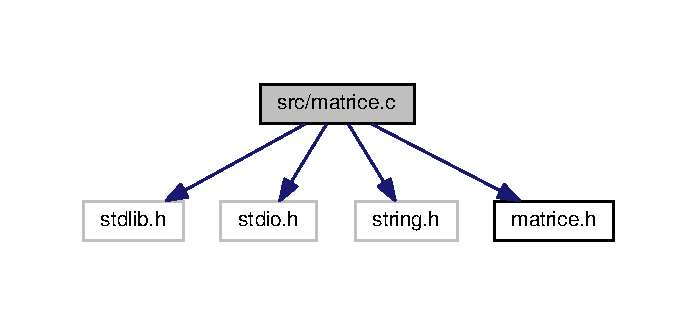
\includegraphics[width=335pt]{matrice_8c__incl}
\end{center}
\end{figure}
\subsection*{Fonctions}
\begin{DoxyCompactItemize}
\item 
\hyperlink{structmat__s}{mat\+\_\+t} \hyperlink{matrice_8c_ad6b0d2064b87d7ad3c6c75956926ee84}{creer\+\_\+matrice} (int ligne, int colonne)
\begin{DoxyCompactList}\small\item\em fonction qui creer et renvoie une matrice de taille ligne colonne \end{DoxyCompactList}\item 
void \hyperlink{matrice_8c_a75eba94bc87bee53fd97eb008b60fd50}{affiche\+\_\+matrice} (\hyperlink{structmat__s}{mat\+\_\+t} ma\+\_\+mat)
\begin{DoxyCompactList}\small\item\em fonction qui affihce la matrice \end{DoxyCompactList}\item 
void \hyperlink{matrice_8c_a778779438efc31f0f0fa189da1833094}{init\+\_\+matrice} (\hyperlink{structmat__s}{mat\+\_\+t} ma\+\_\+mat)
\begin{DoxyCompactList}\small\item\em fonction qui met dans toutes les case de la matrice en parametre \textquotesingle{}0\textquotesingle{} \end{DoxyCompactList}\item 
void \hyperlink{matrice_8c_aa09533da46485f5387d2fd2b411f81b9}{supprim\+\_\+mat} (\hyperlink{structmat__s}{mat\+\_\+t} ma\+\_\+mat)
\begin{DoxyCompactList}\small\item\em fonction qui supprime la matrice \end{DoxyCompactList}\end{DoxyCompactItemize}


\subsection{Description détaillée}
\hyperlink{matrice_8c}{matrice.\+c} comporte toute les fonction utiles a la gestion de la matrice 

\begin{DoxyAuthor}{Auteur}
T\+H\+O\+M\+AS Paul 
\end{DoxyAuthor}
\begin{DoxyVersion}{Version}
1.\+0 
\end{DoxyVersion}
\begin{DoxyDate}{Date}
3 avril 2018 
\end{DoxyDate}


\subsection{Documentation des fonctions}
\index{matrice.\+c@{matrice.\+c}!affiche\+\_\+matrice@{affiche\+\_\+matrice}}
\index{affiche\+\_\+matrice@{affiche\+\_\+matrice}!matrice.\+c@{matrice.\+c}}
\subsubsection[{\texorpdfstring{affiche\+\_\+matrice(mat\+\_\+t ma\+\_\+mat)}{affiche_matrice(mat_t ma_mat)}}]{\setlength{\rightskip}{0pt plus 5cm}{\bf mat\+\_\+t} affiche\+\_\+matrice (
\begin{DoxyParamCaption}
\item[{{\bf mat\+\_\+t}}]{ma\+\_\+mat}
\end{DoxyParamCaption}
)}\hypertarget{matrice_8c_a75eba94bc87bee53fd97eb008b60fd50}{}\label{matrice_8c_a75eba94bc87bee53fd97eb008b60fd50}


fonction qui affihce la matrice 


\begin{DoxyParams}{Paramètres}
{\em ma\+\_\+mat} & est la matrice que l\textquotesingle{}on veut afficher \\
\hline
\end{DoxyParams}
\index{matrice.\+c@{matrice.\+c}!creer\+\_\+matrice@{creer\+\_\+matrice}}
\index{creer\+\_\+matrice@{creer\+\_\+matrice}!matrice.\+c@{matrice.\+c}}
\subsubsection[{\texorpdfstring{creer\+\_\+matrice(int ligne, int colonne)}{creer_matrice(int ligne, int colonne)}}]{\setlength{\rightskip}{0pt plus 5cm}{\bf mat\+\_\+t} creer\+\_\+matrice (
\begin{DoxyParamCaption}
\item[{int}]{ligne, }
\item[{int}]{colonne}
\end{DoxyParamCaption}
)}\hypertarget{matrice_8c_ad6b0d2064b87d7ad3c6c75956926ee84}{}\label{matrice_8c_ad6b0d2064b87d7ad3c6c75956926ee84}


fonction qui creer et renvoie une matrice de taille ligne colonne 


\begin{DoxyParams}{Paramètres}
{\em ligne} & est le nombre de ligne que l\textquotesingle{}on veux dans la matrice \\
\hline
{\em colonne} & est le nombre de colonne que l\textquotesingle{}on veux dans la matrice \\
\hline
\end{DoxyParams}
\begin{DoxyReturn}{Renvoie}
une variable de type mat\+\_\+t \+: une matrice 
\end{DoxyReturn}
\index{matrice.\+c@{matrice.\+c}!init\+\_\+matrice@{init\+\_\+matrice}}
\index{init\+\_\+matrice@{init\+\_\+matrice}!matrice.\+c@{matrice.\+c}}
\subsubsection[{\texorpdfstring{init\+\_\+matrice(mat\+\_\+t ma\+\_\+mat)}{init_matrice(mat_t ma_mat)}}]{\setlength{\rightskip}{0pt plus 5cm}void init\+\_\+matrice (
\begin{DoxyParamCaption}
\item[{{\bf mat\+\_\+t}}]{ma\+\_\+mat}
\end{DoxyParamCaption}
)}\hypertarget{matrice_8c_a778779438efc31f0f0fa189da1833094}{}\label{matrice_8c_a778779438efc31f0f0fa189da1833094}


fonction qui met dans toutes les case de la matrice en parametre \textquotesingle{}0\textquotesingle{} 


\begin{DoxyParams}{Paramètres}
{\em ma\+\_\+mat} & est la matrice que l\textquotesingle{}on veut initialiser \\
\hline
\end{DoxyParams}
\index{matrice.\+c@{matrice.\+c}!supprim\+\_\+mat@{supprim\+\_\+mat}}
\index{supprim\+\_\+mat@{supprim\+\_\+mat}!matrice.\+c@{matrice.\+c}}
\subsubsection[{\texorpdfstring{supprim\+\_\+mat(mat\+\_\+t ma\+\_\+mat)}{supprim_mat(mat_t ma_mat)}}]{\setlength{\rightskip}{0pt plus 5cm}void supprim\+\_\+mat (
\begin{DoxyParamCaption}
\item[{{\bf mat\+\_\+t}}]{ma\+\_\+mat}
\end{DoxyParamCaption}
)}\hypertarget{matrice_8c_aa09533da46485f5387d2fd2b411f81b9}{}\label{matrice_8c_aa09533da46485f5387d2fd2b411f81b9}


fonction qui supprime la matrice 


\begin{DoxyParams}{Paramètres}
{\em ma\+\_\+mat} & est la matrice que l\textquotesingle{}on veut supprimer \\
\hline
\end{DoxyParams}

\hypertarget{mot_8c}{}\section{Référence du fichier src/mot.c}
\label{mot_8c}\index{src/mot.\+c@{src/mot.\+c}}


\hyperlink{mot_8c}{mot.\+c} est un programme qui a les différentes fonction liés a la liste de mot de départ  


{\ttfamily \#include $<$stdlib.\+h$>$}\\*
{\ttfamily \#include $<$stdio.\+h$>$}\\*
{\ttfamily \#include $<$string.\+h$>$}\\*
{\ttfamily \#include \char`\"{}mot.\+h\char`\"{}}\\*
{\ttfamily \#include \char`\"{}outil.\+h\char`\"{}}\\*
{\ttfamily \#include $<$time.\+h$>$}\\*
Graphe des dépendances par inclusion de mot.\+c\+:
\nopagebreak
\begin{figure}[H]
\begin{center}
\leavevmode
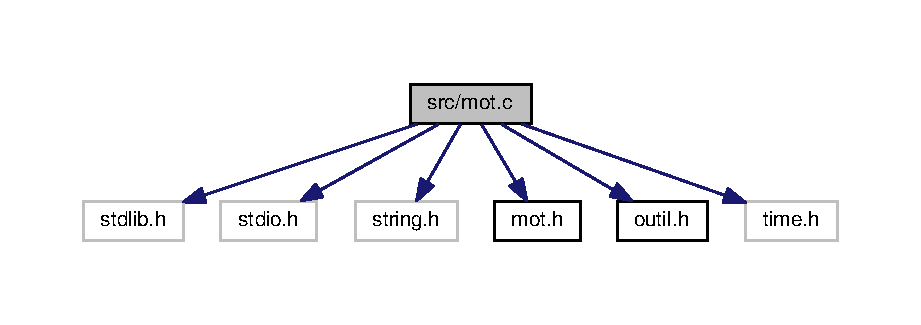
\includegraphics[width=350pt]{mot_8c__incl}
\end{center}
\end{figure}
\subsection*{Fonctions}
\begin{DoxyCompactItemize}
\item 
void \hyperlink{mot_8c_a42ef0fd7fc52130cfabce01e354bafcf}{lire\+\_\+fichier} (void)\hypertarget{mot_8c_a42ef0fd7fc52130cfabce01e354bafcf}{}\label{mot_8c_a42ef0fd7fc52130cfabce01e354bafcf}

\begin{DoxyCompactList}\small\item\em insere dans la liste de mot les mots qui sont dans liste\+\_\+ani.\+txt et ajoute le nombre de mot dans nbmot \end{DoxyCompactList}\item 
void \hyperlink{mot_8c_a2f4a98d1769e42db09aa7f21510fc694}{lire\+\_\+tableau\+\_\+mots} (void)\hypertarget{mot_8c_a2f4a98d1769e42db09aa7f21510fc694}{}\label{mot_8c_a2f4a98d1769e42db09aa7f21510fc694}

\begin{DoxyCompactList}\small\item\em affiche le tableau de mots \end{DoxyCompactList}\item 
char $\ast$ \hyperlink{mot_8c_ad85e71b11082e12b093c501d7e0b6e48}{recup\+\_\+mot} (int i)
\begin{DoxyCompactList}\small\item\em recupère le mot en i (donné en paramètre) \end{DoxyCompactList}\item 
void {\bfseries supprime\+\_\+mot} (int i)\hypertarget{mot_8c_a16b1b712244b17c6c827a76e540af462}{}\label{mot_8c_a16b1b712244b17c6c827a76e540af462}

\item 
int \hyperlink{mot_8c_a5f23001bb152baec608bb8b78cebd03f}{taille\+\_\+mot} (int i)
\begin{DoxyCompactList}\small\item\em return la taille du mot en i (donné en paramètre) \end{DoxyCompactList}\item 
int \hyperlink{mot_8c_a08105e5667c64d7dc196d5ae8491705f}{alea\+\_\+mot} (void)
\begin{DoxyCompactList}\small\item\em return la coordonnée d\textquotesingle{}un mot aléatoire \end{DoxyCompactList}\end{DoxyCompactItemize}
\subsection*{Variables}
\begin{DoxyCompactItemize}
\item 
char $\ast$ {\bfseries tableau\+Mot} \mbox{[}$\,$\mbox{]}\hypertarget{mot_8c_a767dea028f2214af9616d4a8706d83cc}{}\label{mot_8c_a767dea028f2214af9616d4a8706d83cc}

\item 
int {\bfseries nbmot} = 0\hypertarget{mot_8c_a4897be56ba743064cfb43d23397ad6bc}{}\label{mot_8c_a4897be56ba743064cfb43d23397ad6bc}

\end{DoxyCompactItemize}


\subsection{Description détaillée}
\hyperlink{mot_8c}{mot.\+c} est un programme qui a les différentes fonction liés a la liste de mot de départ 

... Documentation ...

\begin{DoxyAuthor}{Auteur}
T\+H\+O\+M\+AS Paul 
\end{DoxyAuthor}
\begin{DoxyVersion}{Version}
1.\+0 
\end{DoxyVersion}
\begin{DoxyDate}{Date}
3 avril 2018 
\end{DoxyDate}


\subsection{Documentation des fonctions}
\index{mot.\+c@{mot.\+c}!alea\+\_\+mot@{alea\+\_\+mot}}
\index{alea\+\_\+mot@{alea\+\_\+mot}!mot.\+c@{mot.\+c}}
\subsubsection[{\texorpdfstring{alea\+\_\+mot(void)}{alea_mot(void)}}]{\setlength{\rightskip}{0pt plus 5cm}int alea\+\_\+mot (
\begin{DoxyParamCaption}
\item[{void}]{}
\end{DoxyParamCaption}
)}\hypertarget{mot_8c_a08105e5667c64d7dc196d5ae8491705f}{}\label{mot_8c_a08105e5667c64d7dc196d5ae8491705f}


return la coordonnée d\textquotesingle{}un mot aléatoire 

\begin{DoxyReturn}{Renvoie}
un int qui est la coordonné du mot 
\end{DoxyReturn}
\index{mot.\+c@{mot.\+c}!recup\+\_\+mot@{recup\+\_\+mot}}
\index{recup\+\_\+mot@{recup\+\_\+mot}!mot.\+c@{mot.\+c}}
\subsubsection[{\texorpdfstring{recup\+\_\+mot(int i)}{recup_mot(int i)}}]{\setlength{\rightskip}{0pt plus 5cm}char $\ast$ recup\+\_\+mot (
\begin{DoxyParamCaption}
\item[{int}]{i}
\end{DoxyParamCaption}
)}\hypertarget{mot_8c_ad85e71b11082e12b093c501d7e0b6e48}{}\label{mot_8c_ad85e71b11082e12b093c501d7e0b6e48}


recupère le mot en i (donné en paramètre) 

supprime le mot en i (donné en paramètre)


\begin{DoxyParams}{Paramètres}
{\em i} & qui représente, la coordonnée dans le tableau ,du mot \\
\hline
\end{DoxyParams}
\begin{DoxyReturn}{Renvoie}
un char $\ast$ qui est le mot
\end{DoxyReturn}

\begin{DoxyParams}{Paramètres}
{\em i} & qui représente ,la coordonnée dans le tableau ,du mot \\
\hline
\end{DoxyParams}
\index{mot.\+c@{mot.\+c}!taille\+\_\+mot@{taille\+\_\+mot}}
\index{taille\+\_\+mot@{taille\+\_\+mot}!mot.\+c@{mot.\+c}}
\subsubsection[{\texorpdfstring{taille\+\_\+mot(int i)}{taille_mot(int i)}}]{\setlength{\rightskip}{0pt plus 5cm}int taille\+\_\+mot (
\begin{DoxyParamCaption}
\item[{int}]{i}
\end{DoxyParamCaption}
)}\hypertarget{mot_8c_a5f23001bb152baec608bb8b78cebd03f}{}\label{mot_8c_a5f23001bb152baec608bb8b78cebd03f}


return la taille du mot en i (donné en paramètre) 


\begin{DoxyParams}{Paramètres}
{\em i} & qui représente, la coordonnée dans le tableau ,du mot \\
\hline
\end{DoxyParams}
\begin{DoxyReturn}{Renvoie}
un int qui est la taille du mot 
\end{DoxyReturn}

\hypertarget{mot__mat_8c}{}\section{Référence du fichier src/mot\+\_\+mat.c}
\label{mot__mat_8c}\index{src/mot\+\_\+mat.\+c@{src/mot\+\_\+mat.\+c}}


\hyperlink{mot__mat_8c}{mot\+\_\+mat.\+c} permet de gerer les \hyperlink{mot__mat_8c}{mot\+\_\+mat.\+c}  


{\ttfamily \#include \char`\"{}mot\+\_\+mat.\+h\char`\"{}}\\*
Graphe des dépendances par inclusion de mot\+\_\+mat.\+c\+:
\nopagebreak
\begin{figure}[H]
\begin{center}
\leavevmode
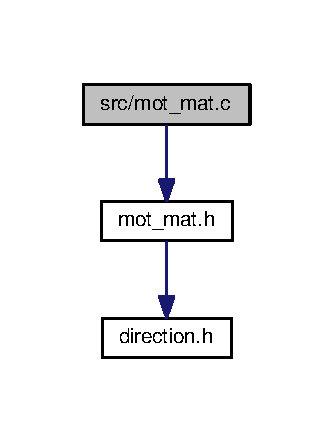
\includegraphics[width=160pt]{mot__mat_8c__incl}
\end{center}
\end{figure}
\subsection*{Fonctions}
\begin{DoxyCompactItemize}
\item 
\hyperlink{structmot__mat__s}{mot\+\_\+mat\+\_\+t} \hyperlink{mot__mat_8c_af9fd8bf5c7ebf73ef478e97f31431729}{creer\+\_\+mot\+\_\+mat} (int colonne, int ligne, char $\ast$mot, t\+\_\+direction direc)
\begin{DoxyCompactList}\small\item\em fonction qui créé un mot\+\_\+mat avec les paramètres donnés \end{DoxyCompactList}\end{DoxyCompactItemize}


\subsection{Description détaillée}
\hyperlink{mot__mat_8c}{mot\+\_\+mat.\+c} permet de gerer les \hyperlink{mot__mat_8c}{mot\+\_\+mat.\+c} 

... Documentation ...

\begin{DoxyAuthor}{Auteur}
T\+H\+O\+M\+AS Paul 
\end{DoxyAuthor}
\begin{DoxyVersion}{Version}
1.\+0 
\end{DoxyVersion}
\begin{DoxyDate}{Date}
3 avril 2018 
\end{DoxyDate}


\subsection{Documentation des fonctions}
\index{mot\+\_\+mat.\+c@{mot\+\_\+mat.\+c}!creer\+\_\+mot\+\_\+mat@{creer\+\_\+mot\+\_\+mat}}
\index{creer\+\_\+mot\+\_\+mat@{creer\+\_\+mot\+\_\+mat}!mot\+\_\+mat.\+c@{mot\+\_\+mat.\+c}}
\subsubsection[{\texorpdfstring{creer\+\_\+mot\+\_\+mat(int colonne, int ligne, char $\ast$mot, t\+\_\+direction direc)}{creer_mot_mat(int colonne, int ligne, char *mot, t_direction direc)}}]{\setlength{\rightskip}{0pt plus 5cm}{\bf mot\+\_\+mat\+\_\+t} creer\+\_\+mot\+\_\+mat (
\begin{DoxyParamCaption}
\item[{int}]{colonne, }
\item[{int}]{ligne, }
\item[{char $\ast$}]{mot, }
\item[{t\+\_\+direction}]{direc}
\end{DoxyParamCaption}
)}\hypertarget{mot__mat_8c_af9fd8bf5c7ebf73ef478e97f31431729}{}\label{mot__mat_8c_af9fd8bf5c7ebf73ef478e97f31431729}


fonction qui créé un mot\+\_\+mat avec les paramètres donnés 


\begin{DoxyParams}{Paramètres}
{\em colonne} & correspond a la colonne ou le mot commence \\
\hline
{\em ligne} & correspond a la ligne ou le mot commence \\
\hline
{\em mot} & correspont au mot qui est dans la matrice \\
\hline
{\em direction} & correspont la direction du mot dans la matrice \\
\hline
\end{DoxyParams}
\begin{DoxyReturn}{Renvoie}
mot\+\_\+mat\+\_\+t une variable qui correspont a un mot dans la matrice 
\end{DoxyReturn}

\hypertarget{outil_8c}{}\section{Référence du fichier src/outil.c}
\label{outil_8c}\index{src/outil.\+c@{src/outil.\+c}}


\hyperlink{outil_8c}{outil.\+c} est une liste de fonction global (qu\textquotesingle{}on pourrais utilsier tel quel dans un autre programme  


{\ttfamily \#include $<$stdlib.\+h$>$}\\*
{\ttfamily \#include $<$stdio.\+h$>$}\\*
{\ttfamily \#include $<$string.\+h$>$}\\*
Graphe des dépendances par inclusion de outil.\+c\+:
\nopagebreak
\begin{figure}[H]
\begin{center}
\leavevmode
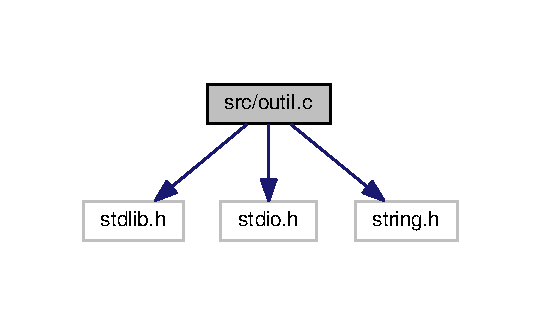
\includegraphics[width=260pt]{outil_8c__incl}
\end{center}
\end{figure}
\subsection*{Fonctions}
\begin{DoxyCompactItemize}
\item 
void \hyperlink{outil_8c_a9e6327c43540dd6ebbfd26fa5ba2f378}{lire\+\_\+tableau} (char $\ast$tableau\mbox{[}$\,$\mbox{]}, int taille)
\begin{DoxyCompactList}\small\item\em affiche un tableau de mot \end{DoxyCompactList}\end{DoxyCompactItemize}


\subsection{Description détaillée}
\hyperlink{outil_8c}{outil.\+c} est une liste de fonction global (qu\textquotesingle{}on pourrais utilsier tel quel dans un autre programme 

... Documentation ...

\begin{DoxyAuthor}{Auteur}
T\+H\+O\+M\+AS Paul 
\end{DoxyAuthor}
\begin{DoxyVersion}{Version}
1.\+0 
\end{DoxyVersion}
\begin{DoxyDate}{Date}
3 avril 2018 
\end{DoxyDate}


\subsection{Documentation des fonctions}
\index{outil.\+c@{outil.\+c}!lire\+\_\+tableau@{lire\+\_\+tableau}}
\index{lire\+\_\+tableau@{lire\+\_\+tableau}!outil.\+c@{outil.\+c}}
\subsubsection[{\texorpdfstring{lire\+\_\+tableau(char $\ast$tableau[], int taille)}{lire_tableau(char *tableau[], int taille)}}]{\setlength{\rightskip}{0pt plus 5cm}lire\+\_\+tableau (
\begin{DoxyParamCaption}
\item[{char $\ast$}]{tableau\mbox{[}$\,$\mbox{]}, }
\item[{int}]{taille}
\end{DoxyParamCaption}
)}\hypertarget{outil_8c_a9e6327c43540dd6ebbfd26fa5ba2f378}{}\label{outil_8c_a9e6327c43540dd6ebbfd26fa5ba2f378}


affiche un tableau de mot 


\begin{DoxyParams}{Paramètres}
{\em tableau} & tableau de mot \\
\hline
{\em taille} & est la taille du tableau \\
\hline
\end{DoxyParams}
\begin{DoxyReturn}{Renvoie}
un int qui est la taille du mot 
\end{DoxyReturn}

%--- End generated contents ---

% Index
\backmatter
\newpage
\phantomsection
\clearemptydoublepage
\addcontentsline{toc}{chapter}{Index}
\printindex

\end{document}
